\documentclass[a4paper]{article}
\usepackage{amsmath}
\usepackage{amsfonts}
\usepackage{amssymb}
\usepackage{graphicx}
\usepackage{float}

\begin{document}

\noindent \large Auteur: Siebe Haché \\
\noindent \large Studierichting: Informatica \\
\noindent \large Oefeningenreeks 5I nr. 2.5 \\

\medskip
\normalsize

Bereken de booglengte $L$ van de functie $f(x) = \dfrac{1}{4}(x^2 - 2\ln x)$ over het interval $[1, e]$. \\

afgeleide: \\

$f'(x) = \dfrac{1}{4} \left( 2x - \dfrac{2}{x} \right) = \dfrac{x}{2} - \dfrac{1}{2x} = \dfrac{x^2 - 1}{2x}$ \\

$1 + (f'(x))^2$: \\

$1 + \left( \dfrac{x^2 - 1}{2x} \right)^2 = 1 + \dfrac{x^4 - 2x^2 + 1}{4x^2}$ \\

$= \dfrac{4x^2 + x^4 - 2x^2 + 1}{4x^2} = \dfrac{x^4 + 2x^2 + 1}{4x^2}$ \\

$= \dfrac{(x^2 + 1)^2}{(2x)^2} = \left( \dfrac{x^2 + 1}{2x} \right)^2$\\

integraal: \\

$L = \displaystyle\int_{1}^{e} \left(\dfrac{x}{2} +\dfrac{1}{2x} \right) dx$ \\

$= \left[ \dfrac{x^2}{4} + \dfrac{1}{2}\ln|x|\right]_{1}^{e}$\\

$= \left( \dfrac{e^2}{4} + \dfrac{1}{2}\ln e\right) - \left( \dfrac{1^2}{4} + \dfrac{1}{2} \ln 1 \right)$ \\

$= \left( \dfrac{e^2}{4} + \dfrac{1}{2} \right) - \left( \dfrac{1}{4} + 0 \right)$\\

$= \dfrac{e^2}{4} + \dfrac{2}{4} - \dfrac{1}{4} = \dfrac{e^2 + 1}{4}$ \\

\begin{figure}[H]
    \centering
    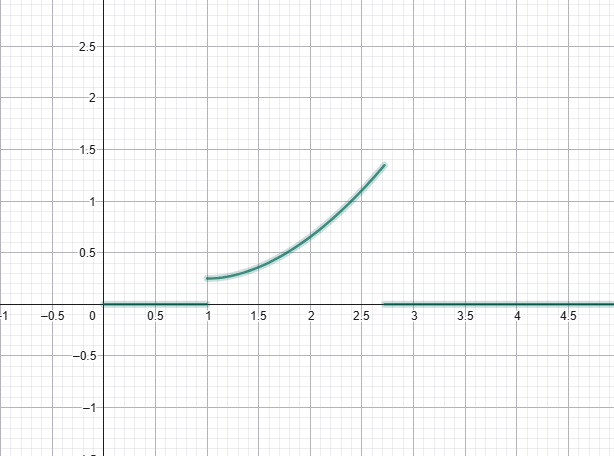
\includegraphics[width=0.6\textwidth]{5I-2.5-siebe.hache.INF.png}
\end{figure}

\begin{thebibliography}{999}
\bibitem{a} Grafiek gemaakt met Geogebra
\end{thebibliography}

\end{document}